\subsection{Modelo}

El modelo es la representación de los datos que maneja el software. Contiene los mecanismos y la lógica necesaria para acceder a la información y para actualizar el estado del modelo. Gráficamente, se podría expresar de la siguiente manera:

\begin{figure}[!h]
    \centering
    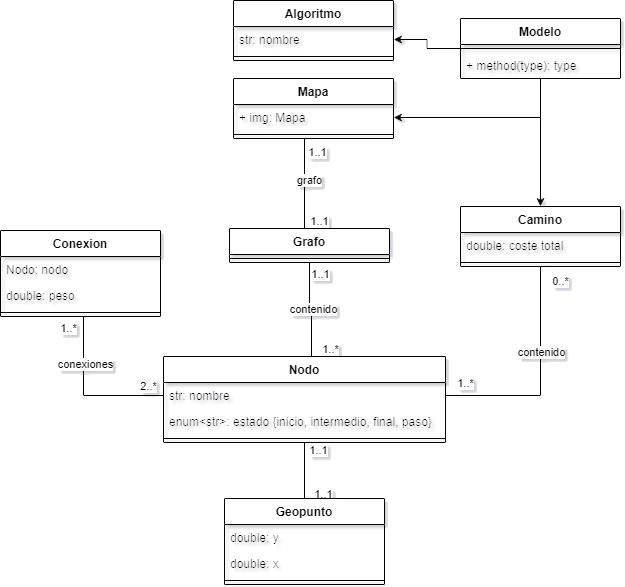
\includegraphics[width=\linewidth]{MVC/Model/img/model.png}
    \caption{Modelo}
    \label{fig:model}
\end{figure}

\begin{description}
\item[Connection] Representa la conexión de un nodo con otro nodo y su peso.
\item[GeoPoint] Representa un punto en el mapa.
\item[Graph] Representa un conjunto de nodos \say{Nodes}
\item[Map] Permite guardar la imagen del mapa con su respectivo grafo
\item[Node] Estructura de datos para guardar los puntos, tiene un identificador, un estado \say{NodeState}, un punto en mapa \say{GeoPoints}, y unas conexiones determinadas con el resto de nodos vecinos \say{Connections}
\item[NodeState] Representa el estado de un nodo
\item[PairPoint] Permite guardar una pareja de \say{GeoPoints}.
\item[Path] Permite guardar una lista de nodos y su coste
\end{description}\bigskip

Finalmente, al ser un módulo de nuestro MVC, implementa la interfaz \texttt{Notify} y su método \texttt{notifyRequest} que le permite recibir notificaciones de los otros módulos del MVC.